\documentclass{standalone}
\usepackage{amsmath}
\usepackage{tikz}
\usetikzlibrary{chains,arrows,shapes}

\newcommand{\PDD}{\ensuremath{\text{PDD}}}
\newcommand{\Hs}{\ensuremath{H_{\text{snow}}}}
\newcommand{\Ms}{\ensuremath{\text{Melt}_{\text{snow}}}}
\newcommand{\Mi}{\ensuremath{\text{Melt}_{\text{ice}}}}

% compile with pdflatex, then run
% convert -density 300 pdd-model-flowchart.pdf -quality 90 pdd-model-flowchart.png

\begin{document}
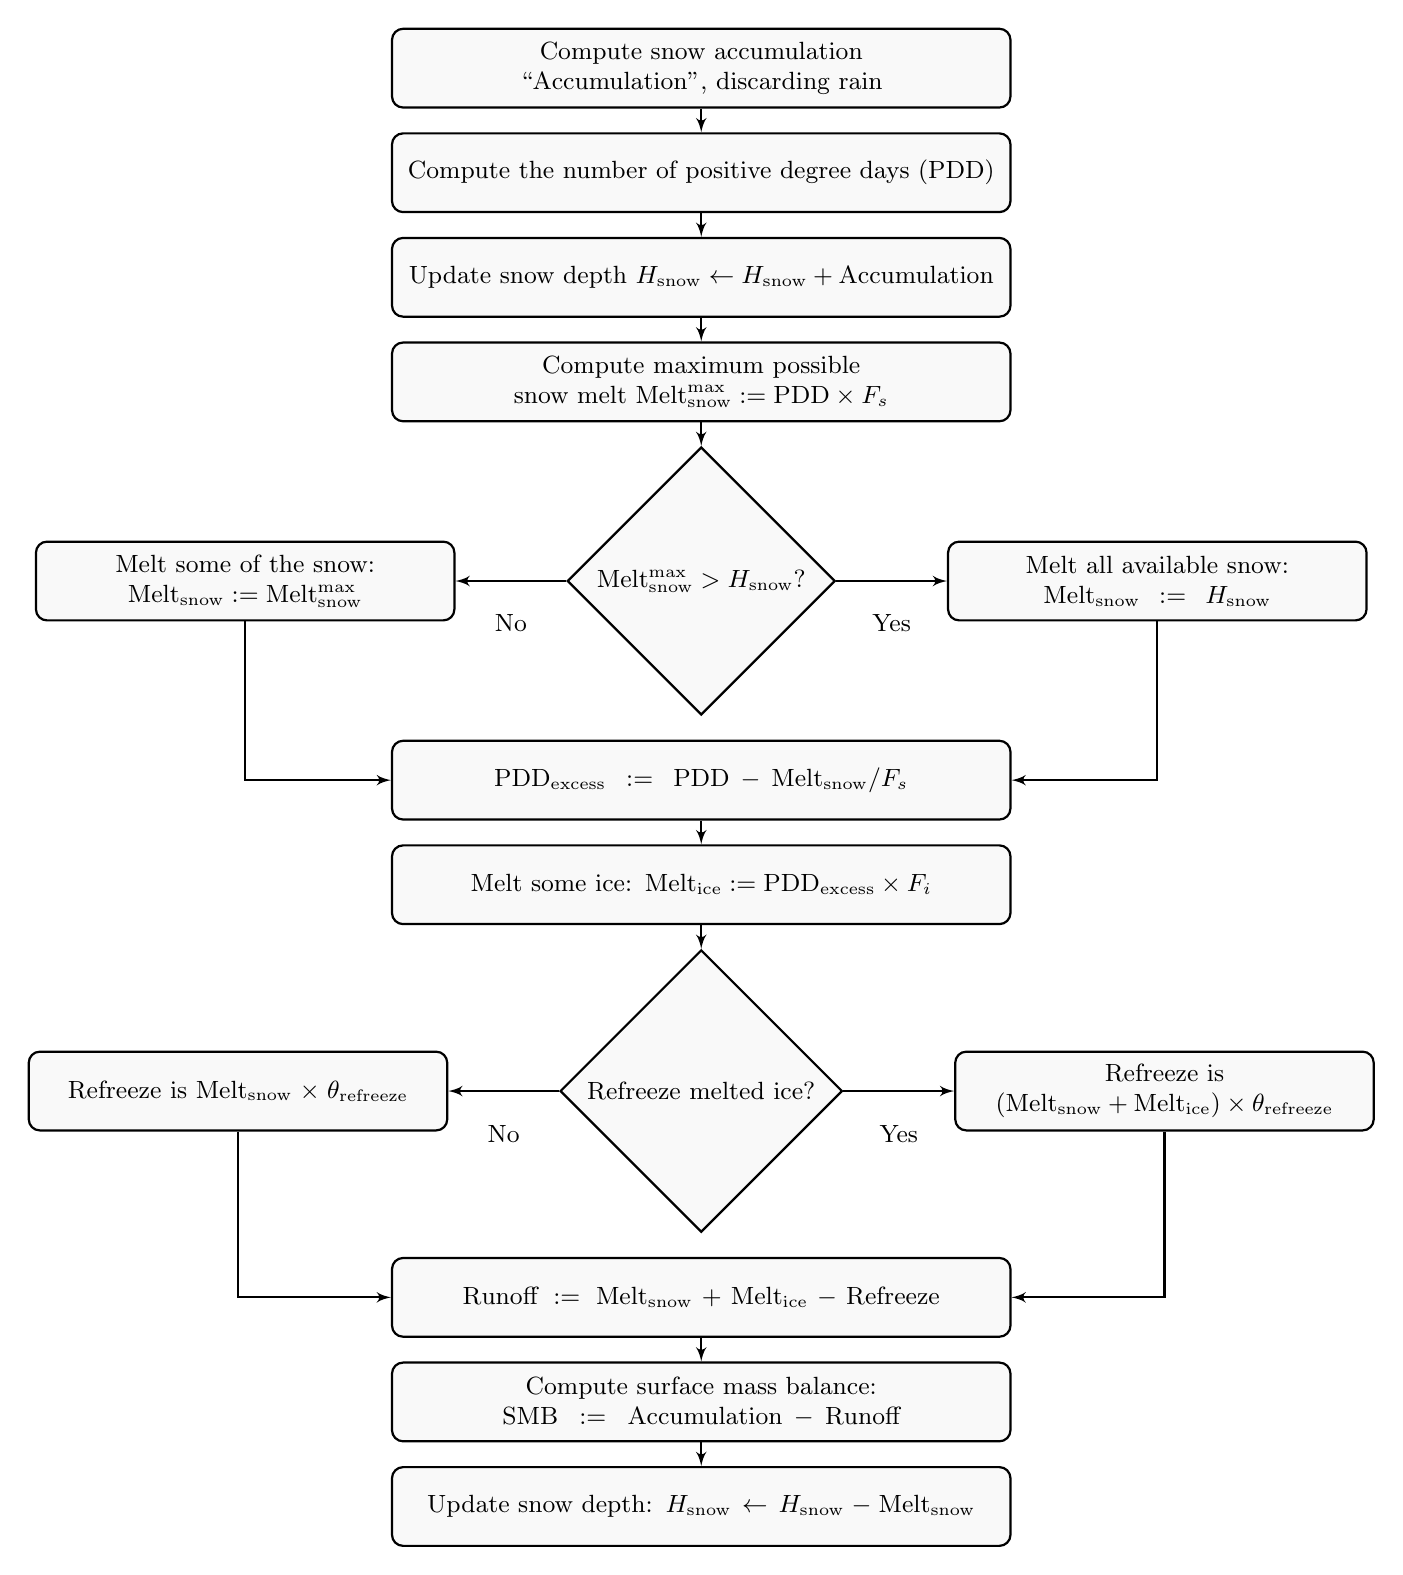
\begin{tikzpicture}[ auto, thick, font=\small, node distance=3mm,
  block/.style={rectangle, rounded corners, draw, fill=gray!5, text width=2in, text centered,
    minimum width=2in, minimum height=1cm},
  big block/.style={block, text width=3in},
  decision/.style={diamond, draw, fill=gray!5},
  line/.style={draw, -latex'},
  start chain=1 going below, every node/.style={on chain},
  every join/.style={-latex'},
  ]

  \node [big block] {Compute snow accumulation \mbox{``Accumulation''}, discarding rain};
  \node [big block, join] {Compute the number of \mbox{positive} degree days (\PDD) };
  \node [big block, join] {Update snow depth \mbox{$\Hs \gets \Hs + \text{Accumulation}$}};
  \node [big block, join] {Compute maximum possible snow melt \mbox{$\Ms^{\text{max}} := \PDD\times F_{s}$}};
  \node (melt all snow) [decision, join] {$\Ms^{\text{max}} > \Hs?$};

  \begin{scope}[start branch=yes, node distance=4em]
    \node (ice melt case) [block, on chain=going right] {\mbox{Melt all available snow:} $\Ms := \Hs$};
  \end{scope}
  \begin{scope}[start branch=no, node distance=4em]
    \node (no ice melt case) [block, on chain=going left] {Melt some of the snow: \mbox{$\Ms := \Ms^{\text{max}}$}};
  \end{scope}

  \node (excess pdds) [big block] {$\PDD_{\text{excess}} := \PDD - \Ms / F_{s}$};
  \node [big block, join] {Melt some ice: \mbox{$\Mi := \PDD_{\text{excess}} \times F_{i}$}};
  \node (refreeze ice) [decision, join] {Refreeze melted ice?};

  \begin{scope}[start branch=yes, node distance=4em]
    \node (refreeze both) [block, on chain=going right] {Refreeze is \mbox{$(\Ms + \Mi) \times \theta_{\text{refreeze}}$}};
  \end{scope}

  \begin{scope}[start branch=no, node distance=4em]
    \node (refreeze snow) [block, on chain=going left] {Refreeze is $\Ms \times \theta_{\text{refreeze}}$};
  \end{scope}

  \node (runoff) [big block] {$\text{Runoff} := \Ms + \Mi - \text{Refreeze}$};
  \node [big block, join] {Compute surface mass balance: $\text{SMB} := \text{Accumulation} - \text{Runoff}$};
  \node [big block, join] {Update snow depth: $\Hs \gets \Hs - \Ms$};
  % special edges:
  \path[line] (melt all snow) -- node {Yes} (ice melt case);
  \path[line] (melt all snow) -- node {No}  (no ice melt case);
  \path[line] (ice melt case) |- (excess pdds);
  \path[line] (no ice melt case) |- (excess pdds);
  \path[line] (refreeze ice) -- node {Yes} (refreeze both);
  \path[line] (refreeze ice) -- node {No}  (refreeze snow);
  \path[line] (refreeze both) |- (runoff);
  \path[line] (refreeze snow) |- (runoff);
\end{tikzpicture}
\end{document}
